\documentclass[12pt,a4paper]{article}
\usepackage[utf8]{inputenc}
\usepackage{graphicx}
\usepackage{hyperref}

\title{World Mobile Node Operations: Architectural Considerations and Best Practices}
\author{Webisoft team}
\date{\today}

\begin{document}
	
	\maketitle
	
	\tableofcontents
	
	\section{Introduction}
	\subsection{Purpose}
	This document outlines the comprehensive architecture of our Decentralized Oracle System, designed to provide secure and reliable cross-chain data validation and transfer.
	
	\subsection{Scope}
	The system encompasses event ingestion, processing, validation, and cross-chain verification mechanisms, along with security measures, governance protocols, and advanced machine learning components.
	
	
	
	
	
	\section{System Overview}
	\subsection{High-Level Architecture}
	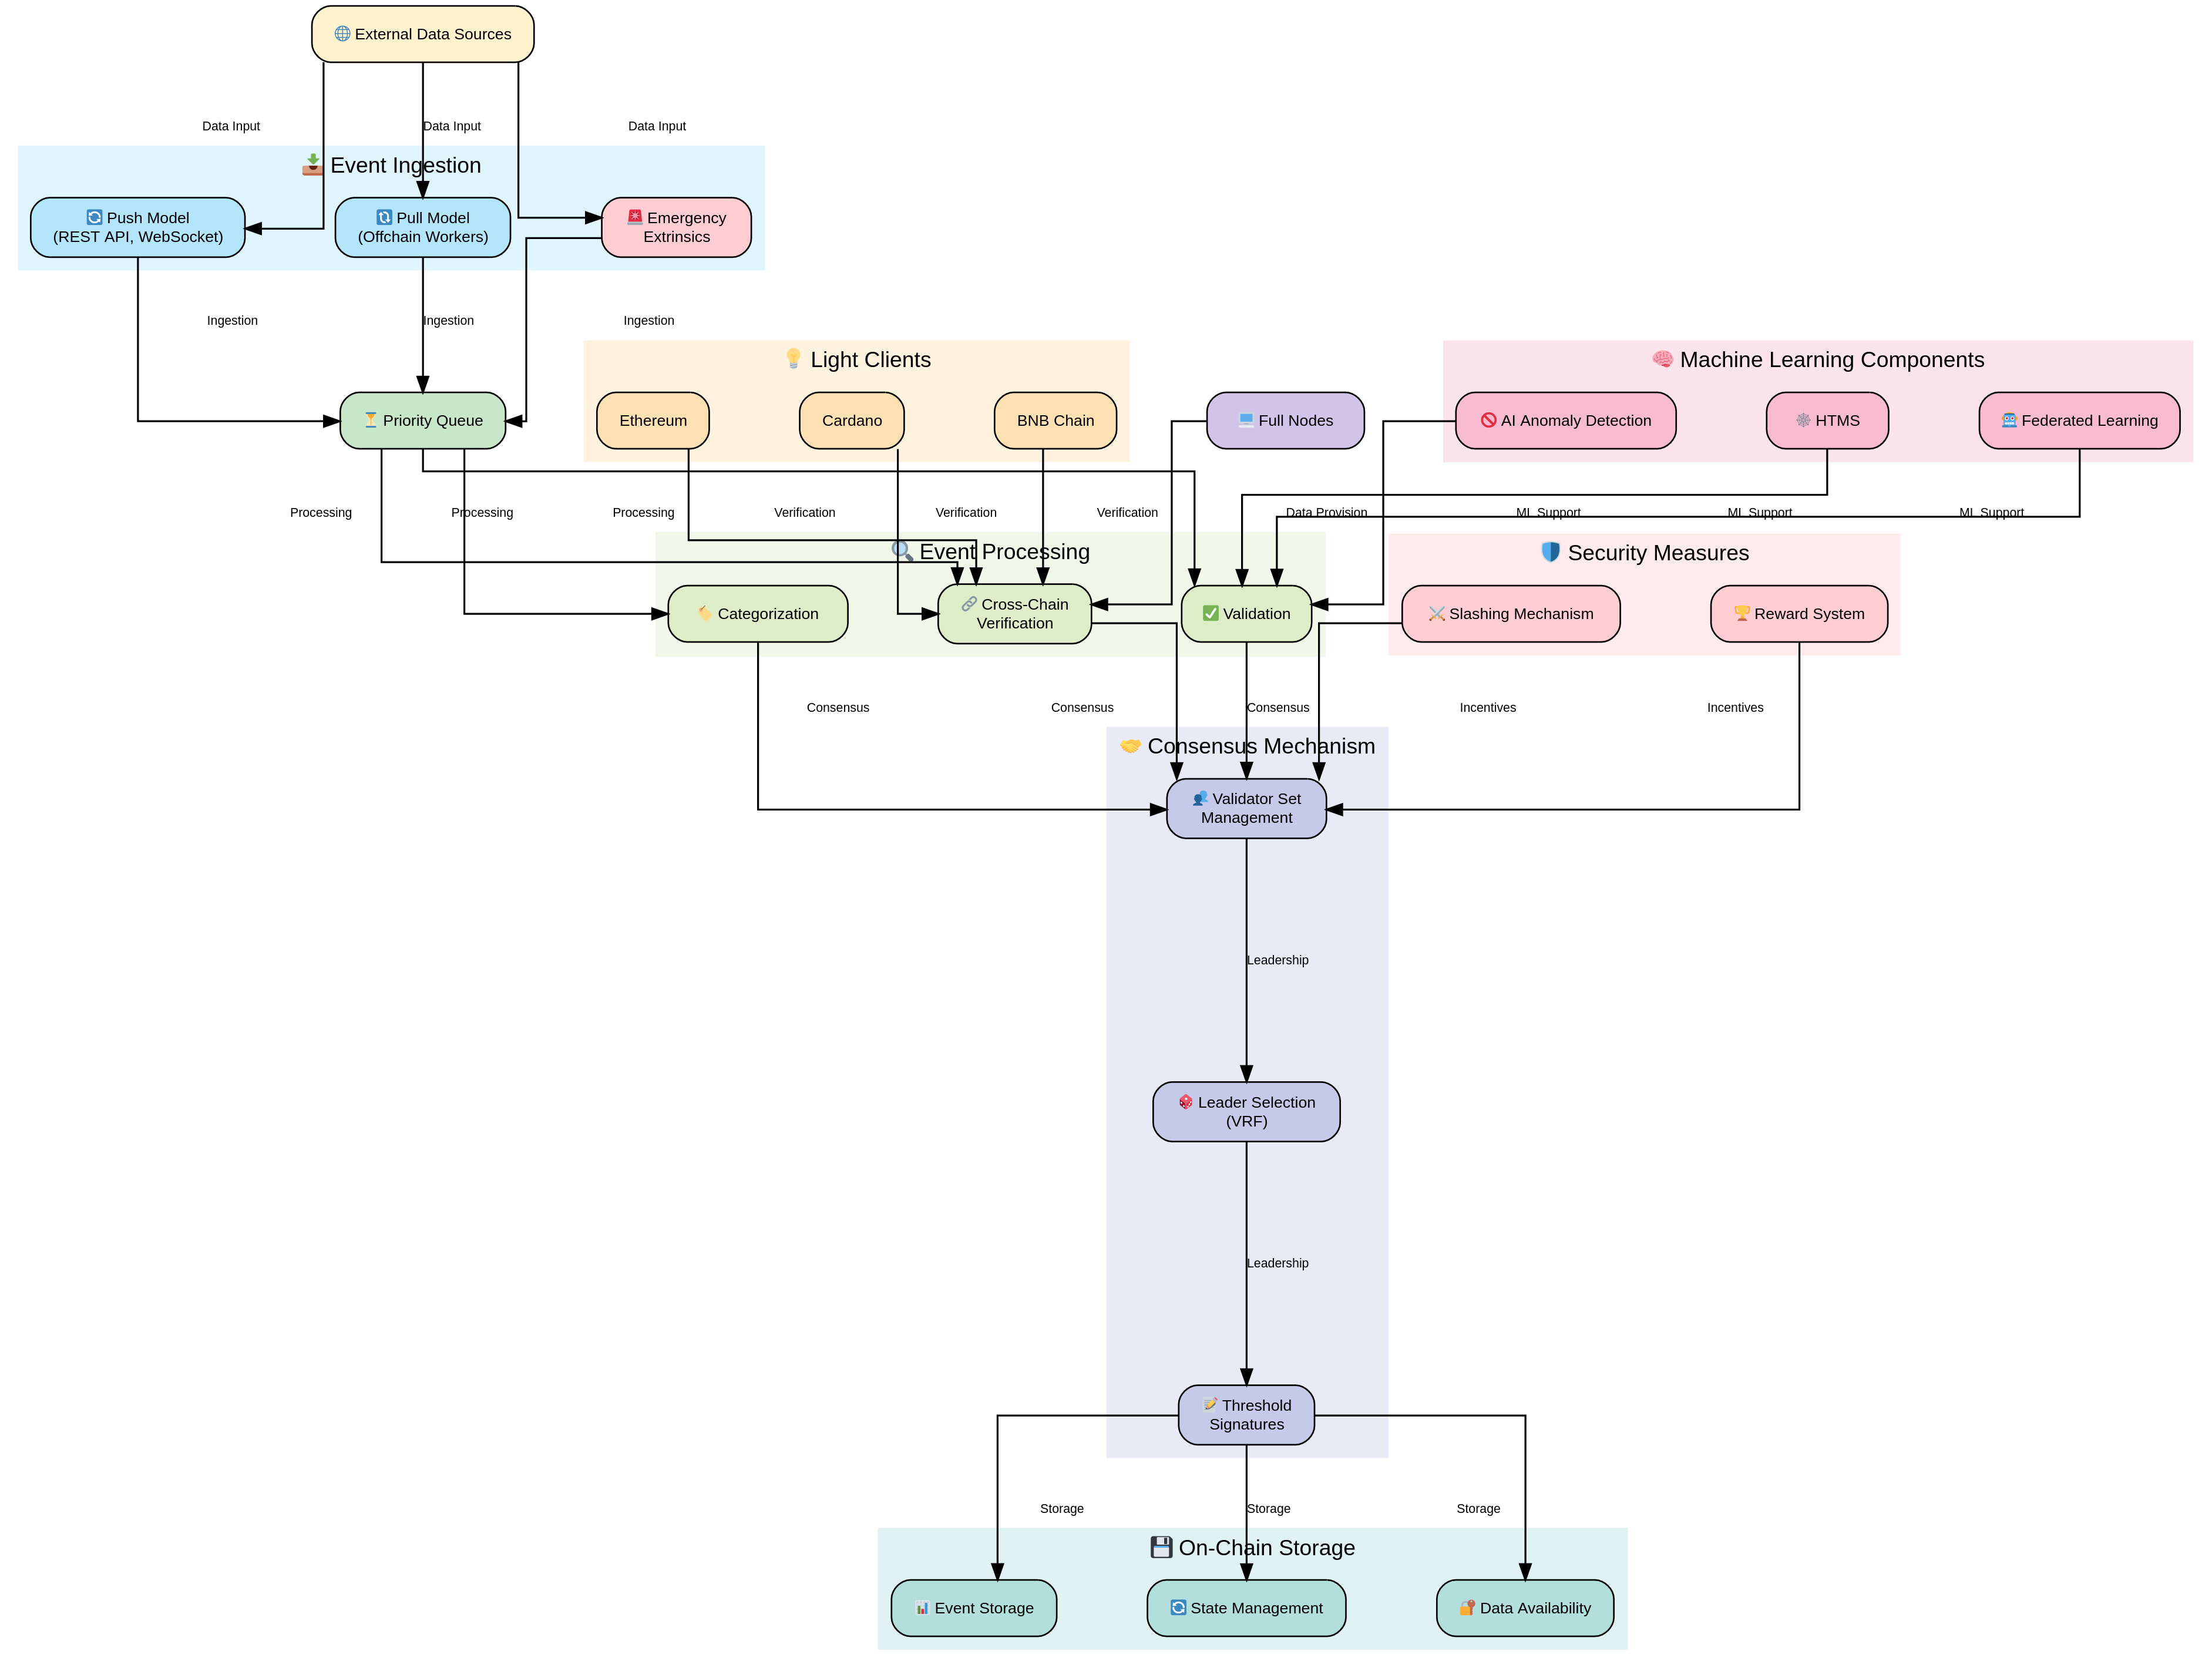
\includegraphics[width=\textwidth]{gen_arch.png}
	
	\section{Core Components}
	\subsection{Event Ingestion}
	The Event Ingestion component is responsible for receiving and initially processing data from various sources before it enters the oracle system. This component implements multiple ingestion models to ensure flexibility and reliability in data acquisition.
	
	\subsubsection{Push Model}
	The Push Model allows external data providers to actively submit events to the oracle system.
	
	\paragraph{Implementation:} 
	\begin{itemize}
		\item REST API endpoints exposed by the oracle nodes
		\item WebSocket connections for real-time data streaming
		\item Rate limiting and authentication mechanisms to prevent abuse
	\end{itemize}
	
	\paragraph{Advantages:}
	\begin{itemize}
		\item Real-time data updates
		\item Reduced load on oracle nodes (no need to constantly poll for data)
		\item Suitable for time-sensitive or sporadic events
	\end{itemize}
	
	\paragraph{Challenges:}
	\begin{itemize}
		\item Needs mechanisms to verify the authenticity of data sources
		\item Potential for malicious data injection
		\item Requires always-on infrastructure to receive pushed data
	\end{itemize}
	
	\subsubsection{Pull Model (Offchain Workers)}
	The Pull Model utilizes Substrate's offchain workers to actively fetch data from external sources at regular intervals.
	
	\paragraph{Implementation:}
	\begin{itemize}
		\item Scheduled offchain workers that run periodically
		\item HTTP clients to fetch data from APIs, websites, or other data sources
		\item Data normalization and initial validation before submission to the oracle system
	\end{itemize}
	
	\paragraph{Advantages:}
	\begin{itemize}
		\item Greater control over data sourcing and update frequency
		\item Can aggregate data from multiple sources before submission
		\item Less vulnerable to malicious data injection
	\end{itemize}
	
	\paragraph{Challenges:}
	\begin{itemize}
		\item May miss real-time updates between scheduled pulls
		\item Increased load on oracle nodes and external data sources
		\item Requires careful management of API rate limits and data source reliability
	\end{itemize}
	
	\subsubsection{Emergency Extrinsics}
	Emergency Extrinsics provide a mechanism for submitting critical, time-sensitive data that bypasses the normal ingestion and queue processes.
	
	\paragraph{Implementation:}
	\begin{itemize}
		\item Special extrinsic type with highest priority in block inclusion
		\item Strict access control, limited to pre-approved accounts or multi-sig transactions
		\item Immediate processing and validation upon receipt
	\end{itemize}
	
	\paragraph{Use Cases:}
	\begin{itemize}
		\item Critical security updates
		\item Emergency halts in DeFi protocols
		\item Urgent governance actions
	\end{itemize}
	
	\paragraph{Security Considerations:}
	\begin{itemize}
		\item Implement a multi-signature requirement for submission
		\item Include automatic circuit breakers to prevent abuse
		\item Maintain detailed audit logs of all emergency submissions
	\end{itemize}
	
	The Event Ingestion component acts as the first line of defense in ensuring data quality and system security. It employs a combination of push and pull models, supplemented by emergency procedures, to provide a robust and flexible data acquisition mechanism for the oracle system.
	
	\subsection{Priority Queue}
	The Priority Queue is a crucial component that manages the ordering and processing of ingested events. It ensures that events are handled efficiently and in the correct order based on their importance and timing.
	
	\subsubsection{Event Ordering}
	Event ordering is critical for maintaining the integrity and timeliness of the oracle system.
	
	\paragraph{Implementation:}
	\begin{itemize}
		\item Use a heap-based priority queue data structure
		\item Assign priority based on event type, timestamp, and source reliability
		\item Implement a decay factor for older events to prevent starvation
	\end{itemize}
	
	\paragraph{Key Features:}
	\begin{itemize}
		\item O(log n) time complexity for insertion and deletion operations
		\item Dynamic priority adjustments based on system load and event criticality
		\item Support for event cancellation and updates
	\end{itemize}
	
	\subsubsection{Rate Limiting}
	Rate limiting prevents system overload and ensures fair usage among different data providers.
	
	\paragraph{Implementation:}
	\begin{itemize}
		\item Token bucket algorithm for flexible rate limiting
		\item Separate rate limits for different event types and sources
		\item Adaptive rate limiting based on system capacity and network conditions
	\end{itemize}
	
	\paragraph{Considerations:}
	\begin{itemize}
		\item Balance between system protection and data freshness
		\item Implement fair queueing to prevent a single source from monopolizing the queue
		\item Provide feedback mechanisms to inform data providers about their current rate limits
	\end{itemize}
	
	The Priority Queue component ensures that the most critical and time-sensitive events are processed first, while also maintaining system stability through intelligent rate limiting. This balancing act is crucial for the overall performance and reliability of the oracle system.
	
	\subsection{Event Processing}
	The Event Processing component is responsible for handling ingested events, validating their content, and preparing them for consensus and on-chain storage. This component plays a critical role in ensuring the accuracy and reliability of the oracle data.
	
	\subsubsection{Categorization}
	Event categorization helps in applying appropriate processing rules and routing events to the correct handlers.
	
	\paragraph{Implementation:}
	\begin{itemize}
		\item Develop a flexible categorization schema to classify events (e.g., financial data, weather data, cross-chain events)
		\item Use machine learning techniques for automatic categorization of complex events
		\item Implement a rule-based system for straightforward event types
	\end{itemize}
	
	\paragraph{Key Features:}
	\begin{itemize}
		\item Dynamic category management to adapt to new event types
		\item Hierarchical categorization for fine-grained processing control
		\item Category-based routing to specialized processing modules
	\end{itemize}
	
	\subsubsection{Validation}
	Validation ensures that the ingested data meets the required quality standards and is free from obvious errors or malicious inputs.
	
	\paragraph{Implementation:}
	\begin{itemize}
		\item Multi-stage validation pipeline (syntax check, schema validation, business rule validation)
		\item Use of cryptographic signatures to verify data origin and integrity
		\item Cross-referencing with historical data and multiple sources for consistency checks
	\end{itemize}
	
	\paragraph{Techniques:}
	\begin{itemize}
		\item Statistical analysis for outlier detection
		\item Smart contract-based validation rules for complex scenarios
		\item AI-powered anomaly detection for sophisticated attack vectors
	\end{itemize}
	
	\subsubsection{Cross-Chain Verification}
	For events originating from or relating to other blockchains, cross-chain verification is essential to ensure data integrity and prevent false information.
	
	\paragraph{Implementation:}
	\begin{itemize}
		\item Integration with light clients of relevant blockchains (Ethereum, Cardano, BNB Chain)
		\item Merkle proof verification for transaction and state root validation
		\item Implementation of chain-specific verification protocols (e.g., Ethereum's block header verification)
	\end{itemize}
	
	\paragraph{Challenges and Solutions:}
	\begin{itemize}
		\item Handling different consensus mechanisms and finality guarantees
		\item Dealing with chain reorganizations and forks
		\item Optimizing verification process for resource-constrained environments
	\end{itemize}
	
	The Event Processing component acts as a crucial filter and enrichment layer, ensuring that only valid, categorized, and verified events proceed to the consensus mechanism and eventual on-chain storage. By implementing robust categorization, validation, and cross-chain verification processes, this component significantly enhances the reliability and trustworthiness of the oracle system.
	
	\section{Consensus Mechanism}
	The Consensus Mechanism is fundamental to the decentralized nature of our oracle system, ensuring that all nodes agree on the validity and order of events. This component is critical for maintaining the integrity and reliability of the oracle data.
	
	\subsection{Validator Set Management}
	Efficient management of the validator set is crucial for the security and performance of the consensus mechanism.
	
	\paragraph{Implementation:}
	\begin{itemize}
		\item Dynamic validator set with entry and exit mechanisms
		\item Stake-based validator selection to align economic incentives
		\item Regular rotation of active validators to prevent centralization
	\end{itemize}
	
	\paragraph{Key Features:}
	\begin{itemize}
		\item Automatic disqualification of misbehaving or underperforming validators
		\item Gradual validator set changes to maintain network stability
		\item Transparent validator metrics and performance tracking
	\end{itemize}
	
	\subsection{Leader Selection (VRF)}
	A fair and unpredictable leader selection process is essential for preventing manipulation and ensuring equitable participation.
	
	\paragraph{Implementation:}
	\begin{itemize}
		\item Verifiable Random Function (VRF) for leader selection
		\item Epoch-based leader rotation to limit the power of any single validator
		\item Backup leader mechanism to handle primary leader failures
	\end{itemize}
	
	\paragraph{Security Considerations:}
	\begin{itemize}
		\item Protection against VRF output manipulation
		\item Resistance to long-range attacks through historical VRF output binding
		\item Mitigation strategies for potential leader collusion
	\end{itemize}
	
	\subsection{Threshold Signatures}
	Threshold signatures provide a way to achieve consensus without requiring every validator to sign every message, improving efficiency and scalability.
	
	\paragraph{Implementation:}
	\begin{itemize}
		\item Use of BLS (Boneh-Lynn-Shacham) signature scheme for efficient threshold signatures
		\item Implementation of (t, n) threshold scheme where t out of n validators are required to produce a valid signature
		\item Distributed Key Generation (DKG) protocol for secure threshold key setup
	\end{itemize}
	
	\paragraph{Advantages:}
	\begin{itemize}
		\item Reduced on-chain storage and verification costs
		\item Improved resistance to certain classes of Byzantine faults
		\item Enablement of more efficient cross-chain verification
	\end{itemize}
	
	\paragraph{Challenges:}
	\begin{itemize}
		\item Complexity of distributed key generation and management
		\item Need for efficient recovery mechanisms in case of validator churn
		\item Balancing the threshold t to optimize between security and liveness
	\end{itemize}
	
	The Consensus Mechanism ensures that all participants in the oracle network reach agreement on the state of the system, including the validity and ordering of events. By combining efficient validator set management, secure leader selection through VRF, and the use of threshold signatures, our system achieves a high degree of decentralization, security, and scalability in its consensus process.
	
	\section{Light Clients}
	Light Clients are essential components of our cross-chain oracle system, enabling efficient and trustless verification of data from other blockchains without the need to run full nodes for each supported chain.
	
	\subsection{Ethereum Light Client}
	The Ethereum Light Client allows our oracle to verify Ethereum state and transaction data efficiently.
	
	\paragraph{Implementation:}
	\begin{itemize}
		\item Use of Ethereum's light client protocol (LES - Light Ethereum Subprotocol)
		\item Implementation of block header verification and merkle proof checking
		\item Storage of recent block headers and state roots for quick verification
	\end{itemize}
	
	\paragraph{Key Features:}
	\begin{itemize}
		\item Efficient syncing of block headers without downloading full blocks
		\item Support for verifying transaction inclusion and account state
		\item Handling of Ethereum's uncle blocks and difficulty adjustments
	\end{itemize}
	
	\paragraph{Challenges:}
	\begin{itemize}
		\item Adapting to Ethereum's transition to Proof of Stake (Ethereum 2.0)
		\item Managing storage growth of accumulated block headers
		\item Handling network upgrades and hard forks
	\end{itemize}
	
	\subsection{Cardano Light Client}
	The Cardano Light Client enables verification of data from the Cardano blockchain, accommodating its unique architecture and consensus mechanism.
	
	\paragraph{Implementation:}
	\begin{itemize}
		\item Adaptation of Cardano's Ouroboros protocol for light client verification
		\item Implementation of stake distribution verification for block producer validation
		\item Support for Cardano's extended UTXO model in state verification
	\end{itemize}
	
	\paragraph{Key Features:}
	\begin{itemize}
		\item Efficient verification of Cardano's epoch boundary blocks
		\item Support for multi-asset ledger state verification
		\item Integration with Cardano's native tokens and smart contract platform
	\end{itemize}
	
	\paragraph{Challenges:}
	\begin{itemize}
		\item Handling Cardano's more complex consensus rules compared to PoW chains
		\item Efficient storage and updating of stake distribution snapshots
		\item Adapting to Cardano's planned protocol upgrades and new features
	\end{itemize}
	
	\subsection{BNB Chain Light Client}
	The BNB Chain Light Client allows for efficient verification of data from the Binance Smart Chain, considering its high throughput and EVM compatibility.
	
	\paragraph{Implementation:}
	\begin{itemize}
		\item Adaptation of Ethereum light client protocols for BNB Chain's modified consensus
		\item Implementation of validator set tracking for BNB Chain's Proof of Staked Authority
		\item Support for BNB Chain's faster block times and finality
	\end{itemize}
	
	\paragraph{Key Features:}
	\begin{itemize}
		\item Quick syncing and verification to match BNB Chain's high throughput
		\item Support for cross-chain bridges between BNB Chain and other networks
		\item Efficient handling of BNB Chain's gas fee model and native token (BNB)
	\end{itemize}
	
	\paragraph{Challenges:}
	\begin{itemize}
		\item Balancing between quick finality and thorough verification
		\item Handling potential divergence between BNB Chain and Ethereum protocols
		\item Efficient storage management due to BNB Chain's high transaction volume
	\end{itemize}
	
	The Light Clients module enables our oracle system to efficiently verify and process data from multiple blockchain networks without the overhead of running full nodes. This approach significantly enhances the oracle's cross-chain capabilities while maintaining a high degree of trustlessness and efficiency.
	
	\section{Running Full Nodes}
	While light clients offer efficiency and reduced resource requirements, running full nodes for supported blockchains provides maximum security and data availability for our oracle system.
	
	\paragraph{Advantages of Full Nodes:}
	\begin{itemize}
		\item Complete verification of all transactions and state transitions
		\item Access to historical data not available to light clients
		\item Ability to participate in network consensus (for supported chains)
	\end{itemize}
	
	\subsubsection{Ethereum Full Node}
	\paragraph{Implementation:}
	\begin{itemize}
		\item Use of Geth (Go Ethereum) or Parity clients
		\item Full synchronization of the entire Ethereum blockchain
		\item Implementation of efficient state pruning to manage storage growth
	\end{itemize}
	
	\paragraph{Considerations:}
	\begin{itemize}
		\item High storage requirements (500GB+ as of 2023)
		\item Significant bandwidth usage for initial sync and ongoing operations
		\item Need for regular software updates to stay compatible with network upgrades
	\end{itemize}
	
	\subsubsection{Cardano Full Node}
	\paragraph{Implementation:}
	\begin{itemize}
		\item Use of Cardano Node software
		\item Full synchronization of the Cardano blockchain
		\item Implementation of stake pool operations for potential participation in block production
	\end{itemize}
	
	\paragraph{Considerations:}
	\begin{itemize}
		\item Moderate storage requirements (50GB+ as of 2023)
		\item Need for understanding Cardano's stake delegation mechanism
		\item Regular updates to accommodate Cardano's planned protocol improvements
	\end{itemize}
	
	\subsubsection{BNB Chain Full Node}
	\paragraph{Implementation:}
	\begin{itemize}
		\item Use of modified Geth client for BNB Chain
		\item Full synchronization of the BNB Chain blockchain
		\item Implementation of validator operations if participating in consensus
	\end{itemize}
	
	\paragraph{Considerations:}
	\begin{itemize}
		\item High storage requirements due to BNB Chain's high transaction volume
		\item Need for high-performance hardware to keep up with rapid block production
		\item Regular updates to stay aligned with BNB Chain's development roadmap
	\end{itemize}
	
	\subsubsection{Integration with Oracle System}
	\paragraph{Implementation:}
	\begin{itemize}
		\item Direct API connections between full nodes and oracle nodes
		\item Implementation of fallback mechanisms to switch between full nodes and light clients
		\item Development of monitoring systems to ensure full node health and synchronization
	\end{itemize}
	
	\paragraph{Challenges:}
	\begin{itemize}
		\item Balancing resource allocation between oracle operations and full node maintenance
		\item Ensuring high availability and fault tolerance for critical full node operations
		\item Managing increased operational complexity and costs associated with running multiple full nodes
	\end{itemize}
	
	While running full nodes requires more resources and maintenance than light clients, it provides the highest level of security and data integrity for our oracle system. The choice between light clients and full nodes can be made based on specific use cases, resource availability, and security requirements.
	
	\section{On-Chain Storage}
	On-Chain Storage is a critical component of our oracle system, responsible for persisting validated data and maintaining the system's state. It ensures that oracle data is immutable, transparent, and easily accessible to smart contracts and other blockchain applications.
	
	\subsubsection{Event Storage}
	Event Storage focuses on efficiently storing and retrieving oracle events on the blockchain.
	
	\paragraph{Implementation:}
	\begin{itemize}
		\item Use of space-efficient data structures (e.g., Merkle trees) for storing event data
		\item Implementation of indexed storage for fast event retrieval
		\item Compression techniques to minimize on-chain storage costs
	\end{itemize}
	
	\paragraph{Key Features:}
	\begin{itemize}
		\item Immutable storage of validated oracle events
		\item Efficient querying capabilities for smart contracts
		\item Support for historical data access and time-based queries
	\end{itemize}
	
	\paragraph{Challenges:}
	\begin{itemize}
		\item Balancing storage efficiency with quick data access
		\item Managing storage growth over time
		\item Ensuring data availability across network participants
	\end{itemize}
	
	\subsubsection{State Management}
	State Management involves maintaining the current state of the oracle system and facilitating state transitions.
	
	\paragraph{Implementation:}
	\begin{itemize}
		\item Use of a state trie structure for efficient updates and proof generation
		\item Implementation of state checkpointing for faster synchronization
		\item Periodic state pruning to manage storage growth
	\end{itemize}
	
	\paragraph{Key Components:}
	\begin{itemize}
		\item Validator set state (current active validators, stakes, performance metrics)
		\item Oracle parameters (e.g., minimum stake, slashing conditions, reward rates)
		\item Cross-chain state (latest verified block headers, bridge contract states)
	\end{itemize}
	
	\paragraph{Optimization Techniques:}
	\begin{itemize}
		\item Lazy evaluation of state changes to reduce unnecessary computations
		\item Caching frequently accessed state data for improved performance
		\item Implementation of state rent mechanisms to incentivize efficient storage usage
	\end{itemize}
	
	\subsubsection{Data Availability}
	Ensuring data availability is crucial for the reliability and usability of the oracle system.
	
	\paragraph{Implementation:}
	\begin{itemize}
		\item Redundant storage across multiple validator nodes
		\item Implementation of data availability proofs
		\item Use of erasure coding for efficient data recovery
	\end{itemize}
	
	\paragraph{Challenges and Solutions:}
	\begin{itemize}
		\item Handling network partitions: Implement eventual consistency mechanisms
		\item Preventing data withholding attacks: Implement challenge-response protocols
		\item Balancing data availability with storage efficiency: Use of off-chain storage solutions with on-chain commitments
	\end{itemize}
	
	The On-Chain Storage component ensures that all critical data in our oracle system is securely and efficiently stored on the blockchain. By implementing robust event storage, state management, and data availability mechanisms, we provide a reliable foundation for the entire oracle ecosystem, enabling trustless and transparent access to validated cross-chain data.
	
	\section{Machine Learning Components}
	\subsection{HTMS (Hierarchical Temporal Memory Systems)}
	Hierarchical Temporal Memory Systems (HTMS) are inspired by the neocortex of the brain and are used to model time-based sequences and make predictions. In the context of our oracle system, HTMS can be employed to analyze and predict trends from the ingested data, enhancing the decision-making processes and providing valuable insights.
	
	\paragraph{Implementation:}
	\begin{itemize}
		\item Use of spatial and temporal pooling algorithms to detect patterns and sequences in data.
		\item Integration with the event ingestion pipeline to continuously learn from the incoming data.
		\item Development of an API for querying HTMS-based predictions and anomalies.
	\end{itemize}
	
	\paragraph{Key Features:}
	\begin{itemize}
		\item Real-time learning and prediction from streaming data.
		\item Anomaly detection to identify unexpected patterns or deviations.
		\item Scalable architecture to handle large volumes of data.
	\end{itemize}
	
	\paragraph{Challenges:}
	\begin{itemize}
		\item Ensuring the accuracy and reliability of predictions in dynamic environments.
		\item Efficiently managing the computational resources for large-scale data processing.
		\item Integrating HTMS with other machine learning and data processing components.
	\end{itemize}
	
	The use of HTMS in our oracle system provides advanced capabilities for real-time analysis and prediction, contributing to the overall intelligence and adaptability of the system.
	
\subsection{Federated Learning}
Federated Learning is a machine learning technique where multiple decentralized devices collaboratively learn a shared model while keeping the training data local. This approach enhances privacy and reduces the need for centralized data storage.

\paragraph{Implementation:}
\begin{itemize}
	\item Design a federated learning protocol to coordinate training across multiple oracle nodes.
\textit{{\tiny 	https://github.com/Paraxiom/federated-learning}}
	\item Implement local training processes on each node, using local event data.
	\item Develop an aggregation mechanism to combine locally trained models into a global model.
	\item Ensure secure communication between nodes for model updates.
\end{itemize}

\paragraph{Key Features:}
\begin{itemize}
	\item Privacy-preserving: No raw data is shared between nodes.
	\item Scalability: Can handle a large number of participating nodes.
	\item Robustness: Reduces the risk of a single point of failure.
\end{itemize}

\paragraph{Challenges:}
\begin{itemize}
	\item Ensuring model convergence despite heterogeneity in local data.
	\item Balancing computation and communication overhead.
	\item Handling unresponsive or malicious nodes.
\end{itemize}

Federated Learning in our oracle system enables the development of powerful machine learning models without compromising the privacy and security of the data, leveraging the distributed nature of the network.
	
	\subsection{AI Anomaly Detection}
	AI Anomaly Detection is crucial for identifying unusual patterns or anomalies in the data that may indicate errors, fraud, or other significant events. This component enhances the reliability and security of the oracle system by providing early warnings about potential issues.
	
	\paragraph{Implementation:}
	\begin{itemize}
		\item Develop and train machine learning models specifically designed for anomaly detection.
		\item Integrate the anomaly detection models with the event processing pipeline.
		\item Implement real-time monitoring and alerting mechanisms for detected anomalies.
		\item Use unsupervised learning techniques to identify anomalies without requiring labeled data.
	\end{itemize}
	
	\paragraph{Key Features:}
	\begin{itemize}
		\item Real-time anomaly detection for immediate response.
		\item Scalability to handle large volumes of data.
		\item Flexibility to adapt to different types of data and evolving patterns.
	\end{itemize}
	
	\paragraph{Challenges:}
	\begin{itemize}
		\item Ensuring a low false-positive rate to avoid unnecessary alerts.
		\item Balancing the detection sensitivity to catch significant anomalies without missing important ones.
		\item Continuously updating the models to adapt to new types of anomalies.
	\end{itemize}
	
	The AI Anomaly Detection component strengthens the oracle system by providing advanced capabilities for identifying and responding to irregularities, thereby maintaining the integrity and trustworthiness of the data.
	
	
	
	\section{Security Measures}
	
	
	\subsection{Slashing Mechanism}
	The slashing mechanism is a crucial component of our decentralized oracle system, designed to disincentivize malicious behavior and ensure the integrity of the network.
	
	\subsubsection{Slashing Conditions}
	\begin{itemize}
		\item \textbf{Double signing}: Validators who sign conflicting blocks or oracle reports.
		\item \textbf{Extended downtime}: Nodes that fail to participate in consensus for a specified period.
		\item \textbf{Invalid data submission}: Validators who submit provably false or manipulated data.
		\item \textbf{Collusion}: Coordinated attempts to manipulate oracle outcomes.
	\end{itemize}
	
	\subsubsection{Slashing Implementation}
	\begin{itemize}
		\item \textbf{Proportional slashing}: The severity of the slash is proportional to the infraction and the validator's stake.
		\item \textbf{Gradual increase}: Repeated infractions result in progressively harsher penalties.
		\item \textbf{Partial slashing}: For minor infractions, only a portion of the stake is slashed to avoid overly punitive measures.
		\item \textbf{Slashing delay}: Implementation of a time delay before slashing to allow for potential reversions or appeals.
	\end{itemize}
	
	\subsubsection{Slashing Distribution}
	\begin{itemize}
		\item \textbf{Burn mechanism}: A portion of slashed tokens is permanently removed from circulation.
		\item \textbf{Redistribution}: Some slashed tokens are redistributed to honest validators as an additional incentive.
		\item \textbf{Insurance fund}: A percentage is allocated to an insurance fund to compensate users in case of major failures.
	\end{itemize}
	
	\subsubsection{Grace Period and Appeals}
	\begin{itemize}
		\item \textbf{Grace period}: Minor, first-time infractions may result in warnings rather than immediate slashing.
		\item \textbf{Appeal process}: Validators can appeal slashing decisions through a decentralized governance mechanism.
		\item \textbf{Evidence submission}: Both accusers and defendants can submit on-chain evidence for evaluation.
	\end{itemize}
	
	\subsubsection{Monitoring and Enforcement}
	\begin{itemize}
		\item \textbf{Automated detection}: Implementation of algorithms to detect slashable offenses in real-time.
		\item \textbf{Whistleblower rewards}: Incentives for network participants to report slashable behavior.
		\item \textbf{Transparency}: All slashing events are recorded on-chain for public verification.
	\end{itemize}
	
	The slashing mechanism plays a vital role in maintaining the security and reliability of our oracle network. By implementing a fair, transparent, and effective slashing system, we ensure that validators are strongly incentivized to act honestly and maintain high-quality service.
	
	\subsection{Reward System}
	The Reward System is a crucial component of our decentralized oracle network, designed to incentivize honest participation, high-quality data provision, and network stability.
	
	\subsubsection{Reward Distribution}
	\begin{itemize}
		\item \textbf{Block rewards}: Validators receive rewards for producing blocks and including oracle data.
		\item \textbf{Oracle fees}: Smart contracts pay fees for accessing oracle data, distributed among data providers and validators.
		\item \textbf{Staking rewards}: Participants earn rewards proportional to their staked tokens.
	\end{itemize}
	
	\subsubsection{Reward Calculation}
	\begin{itemize}
		\item \textbf{Performance-based rewards}: Higher rewards for validators with better uptime and data accuracy.
		\item \textbf{Weighted distribution}: Rewards are weighted based on the stake amount and duration.
		\item \textbf{Dynamic adjustment}: Reward rates adjust based on network participation to maintain economic balance.
	\end{itemize}
	
	\subsubsection{Inflationary Model}
	\begin{itemize}
		\item \textbf{Controlled inflation}: A small inflation rate to fund ongoing rewards and incentivize participation.
		\item \textbf{Deflationary mechanisms}: Partial fee burning to offset inflation and potentially create deflationary pressure.
		\item \textbf{Adaptive issuance}: Adjusting token issuance based on network security needs and economic factors.
	\end{itemize}
	
	\subsubsection{Reputation System}
	\begin{itemize}
		\item \textbf{Reputation scores}: Tracking validator performance over time to influence reward distribution.
		\item \textbf{Historical reliability}: Considering long-term reliability in reward calculations.
		\item \textbf{Reputation recovery}: Mechanisms for validators to recover reputation after unintentional errors.
	\end{itemize}
	
	\subsubsection{Incentive Alignment}
	\begin{itemize}
		\item \textbf{Long-term staking bonuses}: Increased rewards for longer staking periods to promote network stability.
		\item \textbf{Data quality incentives}: Higher rewards for providing high-quality, in-demand data.
		\item \textbf{Participation in governance}: Rewards for active participation in network governance decisions.
	\end{itemize}
	
	\subsubsection{Anti-Gaming Measures}
	\begin{itemize}
		\item \textbf{Sybil resistance}: Reward structure designed to prevent benefits from creating multiple identities.
		\item \textbf{Collusion detection}: Algorithms to identify and penalize coordinated manipulation attempts.
		\item \textbf{Reward caps}: Implementing maximum reward limits to prevent excessive concentration of rewards.
	\end{itemize}
	
	The Reward System is designed to create a sustainable and fair economic model that encourages widespread participation, ensures high-quality oracle services, and maintains the long-term stability and security of the network. By carefully balancing rewards, inflation, and economic incentives, we aim to create a robust and resilient decentralized oracle ecosystem.

	
	\subsection{Privacy-Preserving Event Submission}
	[Content to be developed]

	\subsection{Sybil Attack Prevention}
	Sybil attack prevention is crucial for maintaining the integrity and security of our decentralized oracle network. This section outlines the mechanisms and strategies implemented to deter and mitigate Sybil attacks.
	
	\subsubsection{Stake-Based Participation}
	\begin{itemize}
		\item \textbf{Minimum stake requirement}: Validators must lock up a significant amount of tokens to participate.
		\item \textbf{Stake scaling}: Influence and rewards scale with stake, reducing the effectiveness of creating multiple small-stake identities.
		\item \textbf{Stake slashing}: Malicious behavior results in stake reduction, increasing the cost of attacks.
	\end{itemize}
	
	\subsubsection{Identity Verification}
	\begin{itemize}
		\item \textbf{Proof-of-uniqueness}: Implementation of zero-knowledge proof systems to verify unique identities without compromising privacy.
		\item \textbf{Decentralized identifiers (DIDs)}: Utilization of W3C DID standards for creating verifiable, decentralized digital identities.
		\item \textbf{Reputation-based verification}: Incorporating historical behavior and network interactions into identity assessment.
	\end{itemize}
	
	\subsubsection{Network Structure Analysis}
	\begin{itemize}
		\item \textbf{Graph analysis}: Continuous monitoring of network topology to detect unusual patterns indicative of Sybil behavior.
		\item \textbf{Behavioral clustering}: Grouping nodes based on behavior patterns to identify potential Sybil groups.
		\item \textbf{Temporal analysis}: Examining the timing and sequence of network join events to detect coordinated Sybil attempts.
	\end{itemize}
	
	\subsubsection{Economic Disincentives}
	\begin{itemize}
		\item \textbf{Participation costs}: Implementing transaction fees and computational costs that make large-scale Sybil attacks economically unfeasible.
		\item \textbf{Reward distribution algorithms}: Designing reward mechanisms that do not provide significant advantages to Sybil attackers.
		\item \textbf{Long-term value alignment}: Creating incentives that reward long-term honest participation over short-term manipulation attempts.
	\end{itemize}
	
	\subsubsection{Consensus Mechanism Resilience}
	\begin{itemize}
		\item \textbf{Sybil-resistant leader selection}: Utilizing stake-weighted random selection processes for consensus roles.
		\item \textbf{Quorum diversity requirements}: Ensuring that consensus quorums are not dominated by potentially connected entities.
		\item \textbf{Dynamic difficulty adjustment}: Adapting consensus participation requirements based on network conditions and detected threat levels.
	\end{itemize}
	
	\subsubsection{Ongoing Monitoring and Adaptation}
	\begin{itemize}
		\item \textbf{Anomaly detection systems}: Implementing machine learning models to identify unusual network behaviors indicative of Sybil attacks.
		\item \textbf{Regular security audits}: Conducting thorough reviews of network participants and behaviors to detect long-term, subtle Sybil strategies.
		\item \textbf{Adaptive defense mechanisms}: Continuously updating and improving Sybil resistance techniques based on new attack vectors and network observations.
	\end{itemize}
	
	By implementing these multi-layered Sybil attack prevention mechanisms, our decentralized oracle network maintains its integrity and resistance to manipulation. The combination of economic incentives, technical measures, and ongoing vigilance creates a robust defense against Sybil attacks, ensuring the reliability and trustworthiness of the oracle system.

	\section{Cross-Chain Operations}
	
	\subsection{Block Time and Epoch Management}
	\paragraph{Implementation:}
	\begin{itemize}
		\item Synchronization of different blockchain epochs
		\item Handling of varying block times across chains
		\item Epoch boundary detection and management
	\end{itemize}
	
	\paragraph{Challenges:}
	\begin{itemize}
		\item Dealing with network latency and clock drift
		\item Ensuring consistency across multiple chains
		\item Handling chain reorganizations and forks
	\end{itemize}
	
	\subsection{Finality Guarantees}
	\paragraph{Implementation:}
	\begin{itemize}
		\item Probabilistic vs. deterministic finality across different chains
		\item Wait time determination for adequate finality
		\item Cross-chain finality verification mechanisms
	\end{itemize}
	
	\paragraph{Considerations:}
	\begin{itemize}
		\item Balancing speed and security in cross-chain operations
		\item Handling chains with different finality mechanisms
		\item Mitigating risks of premature finality assumptions
	\end{itemize}
	
	\subsection{State Root Verification}
	\paragraph{Implementation:}
	\begin{itemize}
		\item Merkle proof verification for state transitions
		\item Cross-chain state root commitments
		\item Efficient state synchronization mechanisms
	\end{itemize}
	
	\paragraph{Challenges:}
	\begin{itemize}
		\item Dealing with different state models (UTXO vs. Account-based)
		\item Optimizing storage and computation for state root verifications
		\item Ensuring security against malicious state transition proofs
	\end{itemize}
	
	\subsection{Cross-Chain Data Consistency}
	\paragraph{Implementation:}
	\begin{itemize}
		\item Data normalization across different blockchain formats
		\item Consensus mechanisms for cross-chain data validation
		\item Atomic commitment protocols for cross-chain operations
	\end{itemize}
	
	\paragraph{Key Features:}
	\begin{itemize}
		\item Real-time data consistency checks
		\item Conflict resolution mechanisms for inconsistent data
		\item Scalable architecture for multi-chain data management
	\end{itemize}
	
	\section{Auditability and Dispute Resolution}
	
	\subsection{Logging and Traceability}
	Comprehensive logging and traceability mechanisms are essential for maintaining transparency, facilitating audits, and resolving disputes in our decentralized oracle system.
	
	\paragraph{Implementation:}
	\begin{itemize}
		\item \textbf{Immutable event logs}: All oracle events, including data submissions, validations, and consensus decisions, are recorded on-chain.
		\item \textbf{Cryptographic proofs}: Each logged event includes cryptographic proofs of its authenticity and integrity.
		\item \textbf{Hierarchical logging structure}: Implement a tiered logging system to balance between detail and efficiency.
	\end{itemize}
	
	\paragraph{Key Features:}
	\begin{itemize}
		\item \textbf{Tamper-evident logs}: Any attempt to alter historical logs can be easily detected.
		\item \textbf{Selective disclosure}: Enable privacy-preserving audits through zero-knowledge proofs.
		\item \textbf{Real-time monitoring}: Provide interfaces for real-time system monitoring and alerting.
	\end{itemize}
	
	\paragraph{Challenges and Solutions:}
	\begin{itemize}
		\item \textbf{Storage efficiency}: Implement log compression and pruning strategies to manage long-term storage costs.
		\item \textbf{Query performance}: Develop indexing mechanisms for efficient log querying and analysis.
		\item \textbf{Privacy considerations}: Balance transparency with data protection regulations and user privacy.
	\end{itemize}
	
	\subsection{Dispute Mechanism}
	A robust dispute resolution mechanism is crucial for maintaining trust and fairness in the oracle network, allowing participants to challenge potentially incorrect or malicious data or decisions.
	
	\paragraph{Implementation:}
	\begin{itemize}
		\item \textbf{Dispute initiation}: Any network participant can raise a dispute by staking a minimum amount of tokens.
		\item \textbf{Evidence submission}: Both the disputer and the challenged party can submit evidence on-chain.
		\item \textbf{Tiered resolution process}: Implement a multi-level dispute resolution system, starting with automated checks and escalating to community voting if necessary.
	\end{itemize}
	
	\paragraph{Key Features:}
	\begin{itemize}
		\item \textbf{Time-bound resolution}: Each stage of the dispute process has a defined time limit to ensure timely resolutions.
		\item \textbf{Incentive alignment}: Correct dispute outcomes are rewarded, while frivolous disputes are penalized.
		\item \textbf{Transparency}: All dispute proceedings and outcomes are publicly visible and verifiable.
	\end{itemize}
	
	\paragraph{Dispute Categories:}
	\begin{itemize}
		\item \textbf{Data accuracy disputes}: Challenges to the correctness of oracle data.
		\item \textbf{Consensus disputes}: Disagreements about the validity of consensus decisions.
		\item \textbf{Slashing disputes}: Appeals against slashing decisions.
		\item \textbf{Governance disputes}: Challenges to the outcome of governance votes.
	\end{itemize}
	
	\paragraph{Challenges and Mitigations:}
	\begin{itemize}
		\item \textbf{Sybil resistance}: Implement stake-weighted voting in community-level dispute resolution.
		\item \textbf{Expert resolution}: For highly technical disputes, incorporate a mechanism to involve subject matter experts.
		\item \textbf{Appeal process}: Allow for appeals of dispute outcomes under specific conditions to ensure fairness.
	\end{itemize}
	
	The combination of comprehensive logging and a fair dispute resolution mechanism ensures the auditability and accountability of our oracle system, fostering trust among participants and users.
	
\section{Security Hardening}

\subsection{Cross-Chain Security Challenges}
\paragraph{Unique Risks:}
\begin{itemize}
	\item \textbf{Bridge vulnerabilities}: Highlighting recent high-profile bridge hacks and their impact.
	\item \textbf{Finality discrepancies}: Risks associated with different finality mechanisms across chains.
	\item \textbf{Replay attacks}: Potential for transaction replay across different networks.
\end{itemize}

\subsection{Advanced Cryptographic Techniques}
\paragraph{Implementation:}
\begin{itemize}
	\item \textbf{Post-quantum cryptography}: Preparing for quantum-resistant algorithms.
	\item \textbf{Threshold cryptography}: Enhancing key management and signature schemes.
	\item \textbf{Homomorphic encryption}: Enabling computations on encrypted data for enhanced privacy.
\end{itemize}

\subsection{Formal Verification}
\paragraph{Approach:}
\begin{itemize}
	\item \textbf{Smart contract verification}: Rigorous mathematical proofs of contract correctness.
	\item \textbf{Protocol-level verification}: Ensuring the soundness of cross-chain communication protocols.
	\item \textbf{Automated theorem proving}: Leveraging tools for continuous verification of system properties.
\end{itemize}

\subsection{Bounded Vectors and Resource Limits}
\paragraph{Implementation:}
\begin{itemize}
	\item \textbf{Static analysis}: Enforcing bounds on vector sizes and loop iterations.
	\item \textbf{Resource metering}: Implementing fine-grained controls on computation and storage usage.
	\item \textbf{Panic handling}: Graceful error management for out-of-bound operations.
\end{itemize}

\subsection{No-std Implementation}
\paragraph{Benefits:}
\begin{itemize}
	\item \textbf{Reduced attack surface}: Minimizing dependencies to reduce potential vulnerabilities.
	\item \textbf{WASM compatibility}: Ensuring core components can run in WebAssembly environments.
	\item \textbf{Embedded systems support}: Enabling oracle functionality on resource-constrained devices.
\end{itemize}

\subsection{Continuous Security Audits}
\paragraph{Process:}
\begin{itemize}
	\item \textbf{Regular third-party audits}: Scheduling comprehensive security reviews by expert firms.
	\item \textbf{Automated scanning}: Implementing continuous vulnerability scanning and static analysis tools.
	\item \textbf{Bug bounty programs}: Engaging the wider security community to identify potential vulnerabilities.
\end{itemize}

\subsection{Incident Response and Recovery}
\paragraph{Preparation:}
\begin{itemize}
	\item \textbf{Incident response playbooks}: Developing detailed plans for various attack scenarios.
	\item \textbf{Emergency shutdown procedures}: Implementing mechanisms for rapid system pausing in case of detected attacks.
	\item \textbf{State recovery mechanisms}: Designing systems for rollback and recovery of compromised state.
\end{itemize}

The security hardening process is continuous and critical, especially in the context of cross-chain operations where the stakes are exceptionally high. By implementing these advanced security measures, we aim to create a robust and resilient oracle system that can withstand the unique challenges of operating across multiple blockchain environments.
	
\section{Conclusion}

This comprehensive architecture document outlines the intricate design of our Decentralized Oracle System, a cutting-edge solution aimed at providing secure and reliable cross-chain data validation and transfer. The scope and depth of this system underscore the complexity involved in building a robust, decentralized infrastructure for the evolving blockchain ecosystem.

\paragraph{Key Architectural Components:}
\begin{itemize}
	\item Event Ingestion and Processing mechanisms ensuring data quality and reliability
	\item Advanced Consensus Mechanisms leveraging VRF and threshold signatures
	\item Light Clients and Full Node integration for efficient cross-chain operations
	\item On-Chain Storage solutions optimized for blockchain environments
	\item Machine Learning Components enhancing system intelligence and adaptability
	\item Robust Security Measures including slashing mechanisms and Sybil attack prevention
	\item Cross-Chain Operations handling the intricacies of multi-chain interactions
	\item Comprehensive Auditability and Dispute Resolution processes
	\item Rigorous Security Hardening practices addressing the unique challenges of decentralized systems
\end{itemize}

The decentralized nature of this oracle system, combined with its cross-chain capabilities, presents unique challenges that require innovative solutions. The integration of advanced cryptographic techniques, machine learning components, and robust security measures reflects the cutting-edge approach necessary for such a system.

It is crucial to recognize that the development and implementation of this system is a significant undertaking. The complexity of cross-chain operations, the need for impeccable security, and the requirement for high reliability demand substantial resources, expertise, and time. 

Moreover, the rapidly evolving nature of blockchain technology necessitates an adaptable and forward-thinking approach. As new blockchain platforms emerge and existing ones evolve, our oracle system must be flexible enough to accommodate these changes while maintaining its core functionality and security.

The security hardening section, in particular, highlights the critical importance of robust security measures in cross-chain environments. Recent high-profile incidents in the blockchain space, especially involving cross-chain bridges, serve as stark reminders of the high stakes involved and the necessity for rigorous security practices.

In conclusion, this Decentralized Oracle System represents a significant advancement in blockchain interoperability and data reliability. Its successful implementation will require careful planning, expert execution, and ongoing maintenance and upgrades. The potential impact of such a system on the blockchain ecosystem is substantial, enabling new levels of cross-chain interaction and data integrity that can drive the next wave of blockchain adoption and innovation.

As we move forward with this project, it will be essential to maintain a clear focus on security, scalability, and adaptability. The architecture outlined in this document provides a solid foundation, but the journey from architecture to implementation will require dedicated effort, continuous learning, and a commitment to excellence in every aspect of the system's development and operation.
	
\end{document}
